\chapter{LHCとATLAS実験}\label{chapter2}
本章では、Run-3における大型ハドロン衝突型加速器であるLHC加速器とATLAS検出器の概要について述べる。


\section{LHC加速器}\label{section2-1}
LHCは周長27kmの陽子陽子衝突型大型円形加速器であり、スイスのジュネーブ郊外にあるCERN地下100mに設置されている。LHCの全体図を図~\ref{fig:2-1}に示す。LHCは重心系エネルギー14TeV、瞬間ルミノシティ1.0$\times10^{34}$cm$^{-2}$s$^{-1}$での陽子陽子衝突が可能なように設計されている。ルミノシティとはどれほど多くの衝突データを得られるかの指標として用いられる値で、毎秒・単位断面積当たり(cm$^{-2}$s$^{-1}$)のパートン衝突頻度であり、これを一定期間において積分したものを積分ルミノシティと呼ぶ。

\begin{figure}[h]
  \centering
  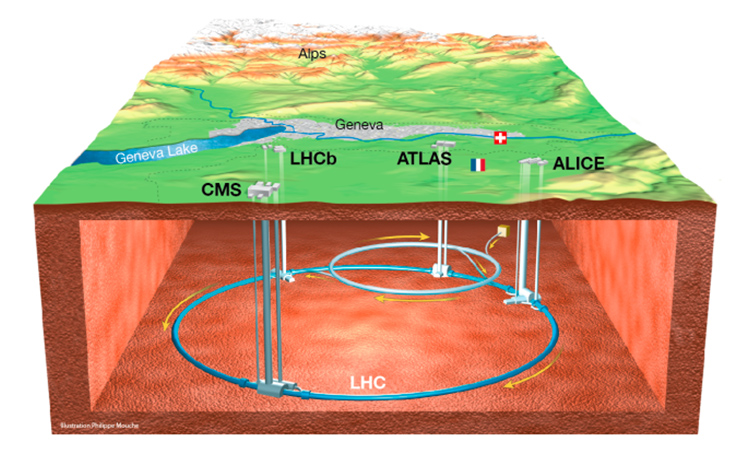
\includegraphics[clip, width=11cm]{fig/2/lhc_map.jpg}
  \caption{LHC加速器の全体図\cite{article:Overall_view_LHC}。地下100mに設置されたLHCの4つ衝突点にそれぞれ検出器が配置されている。}
  \label{fig:2-1}
\end{figure}

LHCでは陽子はバンチと呼ばれる塊で2本のリングで互いに逆向きに加速されており、バンチが連なることでビームを形成している。加速リング内には、超伝統電磁石によって最大8.33Tの磁場がかけられ、磁場によって陽子が曲げられ加速リング内を周回する。ビームを交差させることによって、25nsおきに陽子陽子衝突を起こしている。
LHCの陽子陽子衝突点は全部で4か所あり、それぞれで実験が行われている。ATLAS~(A~Troidal~LHC~ApparatuS)、CMS~(Compact~Muon~Solenoid)\cite{article:CMSExperiment}では大型汎用検出器を用いて、標準模型の精密測定や新物理の探索など幅広い物理を対象とした研究が行われている。また、LHCb~(Large~Hadron~COllider-b)\cite{article:LHCbExperiment}ではビームライン付近に感度を持つ検出器を設置することでbクォークの物理を対象とした研究が行われており、ALICE~(A~Large~Ion~Collider~Experiment)\cite{article:ALICEExperiment}は重イオンを用いた衝突実験で、鉛原子核を加速させ、高エネルギー領域での衝突によって生じるクォーク・グルーオンプラズマを対象とした研究を行っている。
CERNに設置されている加速器・検出器群を図~\ref{fig:2-2}に示す。

\begin{figure}[h]
  \centering
  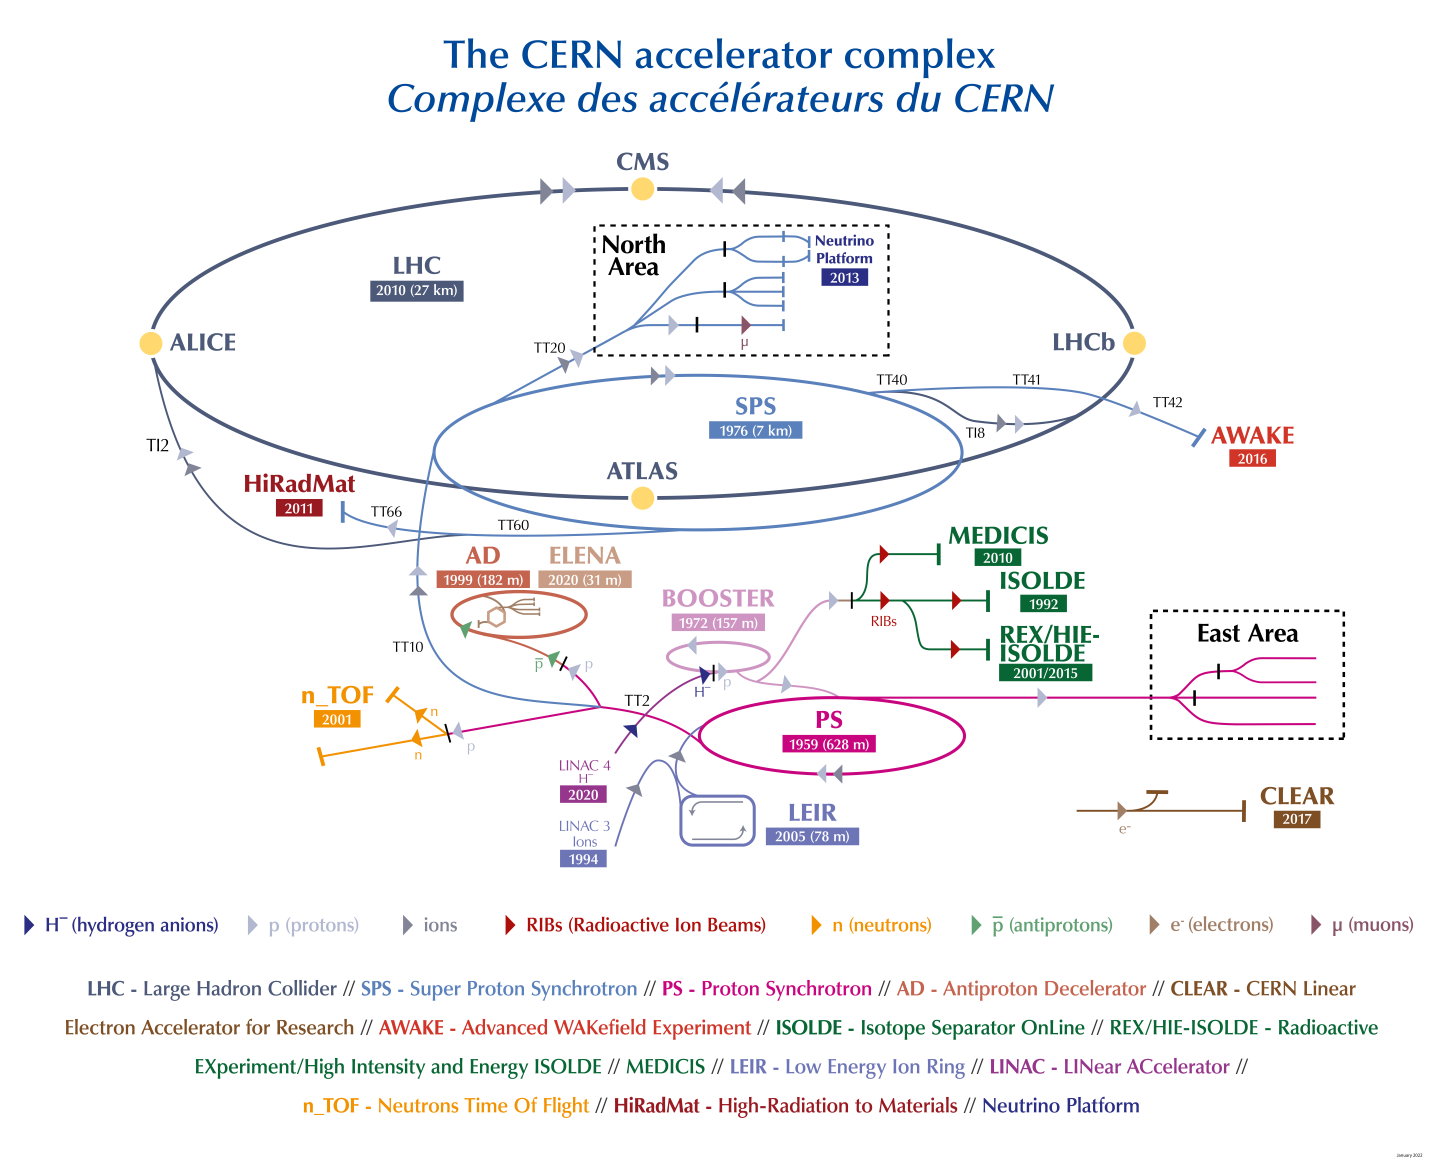
\includegraphics[clip, width=11cm]{fig/2/accel_complex-v2022_complex.png}
  \caption{CERNに設置されている加速器・検出器群\cite{article:accelerator-complex}}
  \label{fig:2-2}
\end{figure}


図~\ref{fig:2-3}にLHCの運転計画を示す。
LHCは第1期運転~(Run-1)として2010年から本格的に運転を開始し、7TeVから8TeVの重心系エネルギー($\sqrt{s}$)で2012年まで稼働した。最高瞬間ルミノシティは0.77$\times10^{34}$cm$^{-2}$s$^{-1}$であった。その後、2013年から2015年までのシャットダウン期間~(LS1)で加速器のアップグレードを行い、2015年から2018年までRun-2として最高瞬間ルミノシティ2.0$\times10^{34}$cm$^{-2}$s$^{-1}$、積分ルミノシティ約$150fb^{-1}$で運転が行われた。2019年から再びシャットダウン期間~(LS2)となり、2022初旬まで加速器のアップグレードが行われた。2022年7月よりRun-3としてデータ取得が開始され、2025年まで重心系エネルギーを13.6TeV、瞬間ルミノシティを2.0$\times10^{34}$cm$^{-2}$s$^{-1}$で運転を行い積分ルミノシティ350fb$^{-1}$のデータ取得を目指している。
また、アップグレードを経て2029年からより高いルミノシティでの高輝度LHC実験(HL-LHC)の運転が予想されている。

\begin{figure}[h]
  \centering
  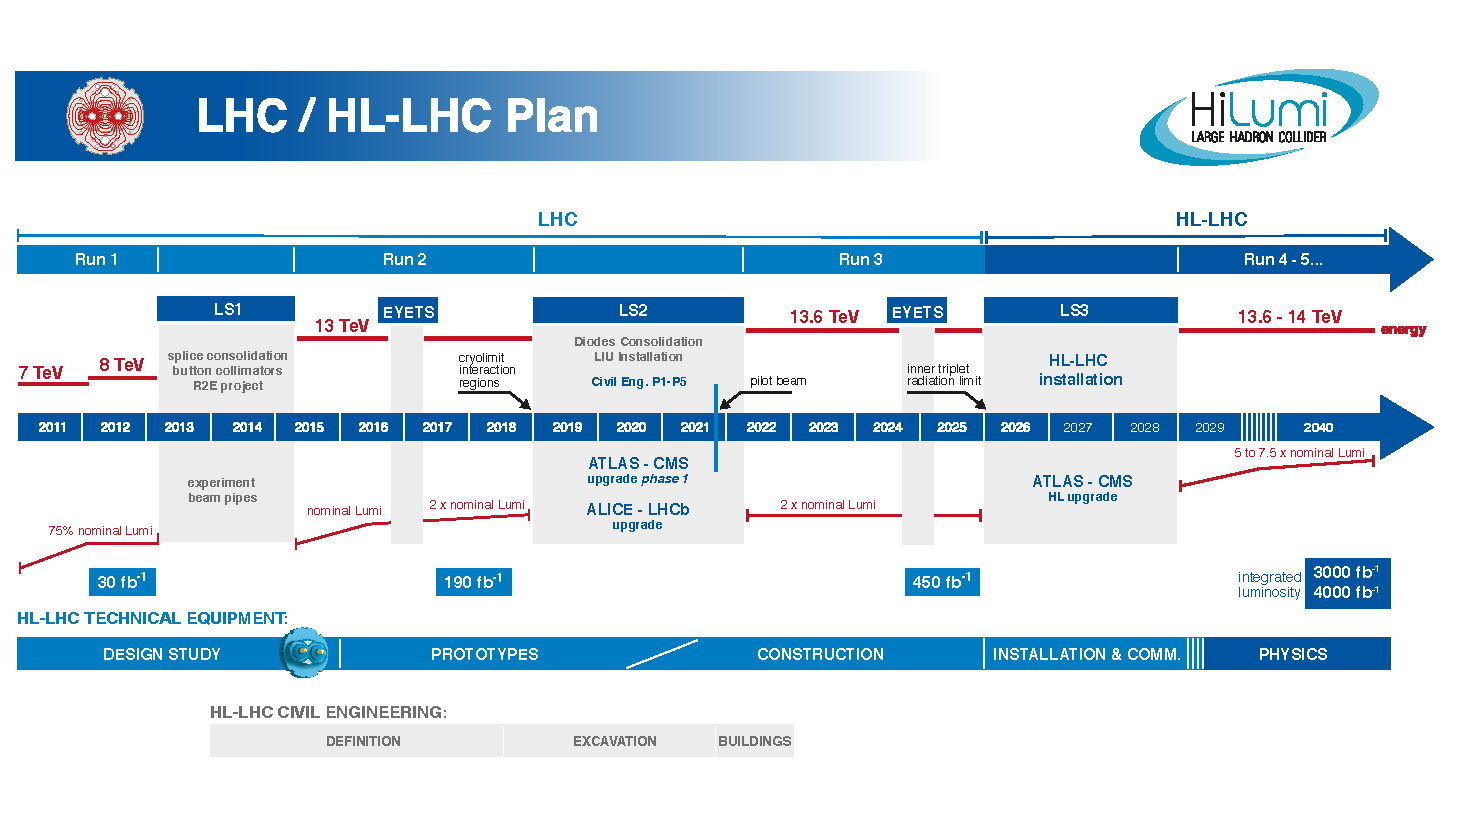
\includegraphics[clip, width=11cm]{fig/2/HL-LHC_Janvier2022.pdf}
  \caption{LHCの運転とアップグレード計画\cite{article:LHCDesignReport}}
  \label{fig:2-3}
\end{figure}



\section{ATLAS検出器}\label{section2-2}

ATLAS検出器は、LHCの衝突点の1つに設置された、直径25m、長さ44mの円筒形の大型汎用検出器である\cite{Aad:1129811}。ATLAS 検出器の全体像を図~\ref{fig:2-4}に示す。
ATLAS実験では様々な物理を研究対象としているので、陽子陽子衝突によって出てくる様々な粒子の種類やエネルギー・運動量を精密に測定できるように設計されている。
ATLAS検出器は複数の検出器を組み合わせて構成されており、内側から内部飛跡検出器、カロリメータ、ミューオン検出器といった検出器が設置されている。また、内部飛跡検出器とカロリメータの間には超伝導ソレノイド磁石、カロリメータの外側にはトロイド磁石がそれぞれ設置されている。
これらの検出器から得られる情報を組み合わせることで、粒子識別や粒子のエネルギーなどの測定を行っている。

\begin{figure}[tb]
  \centering
  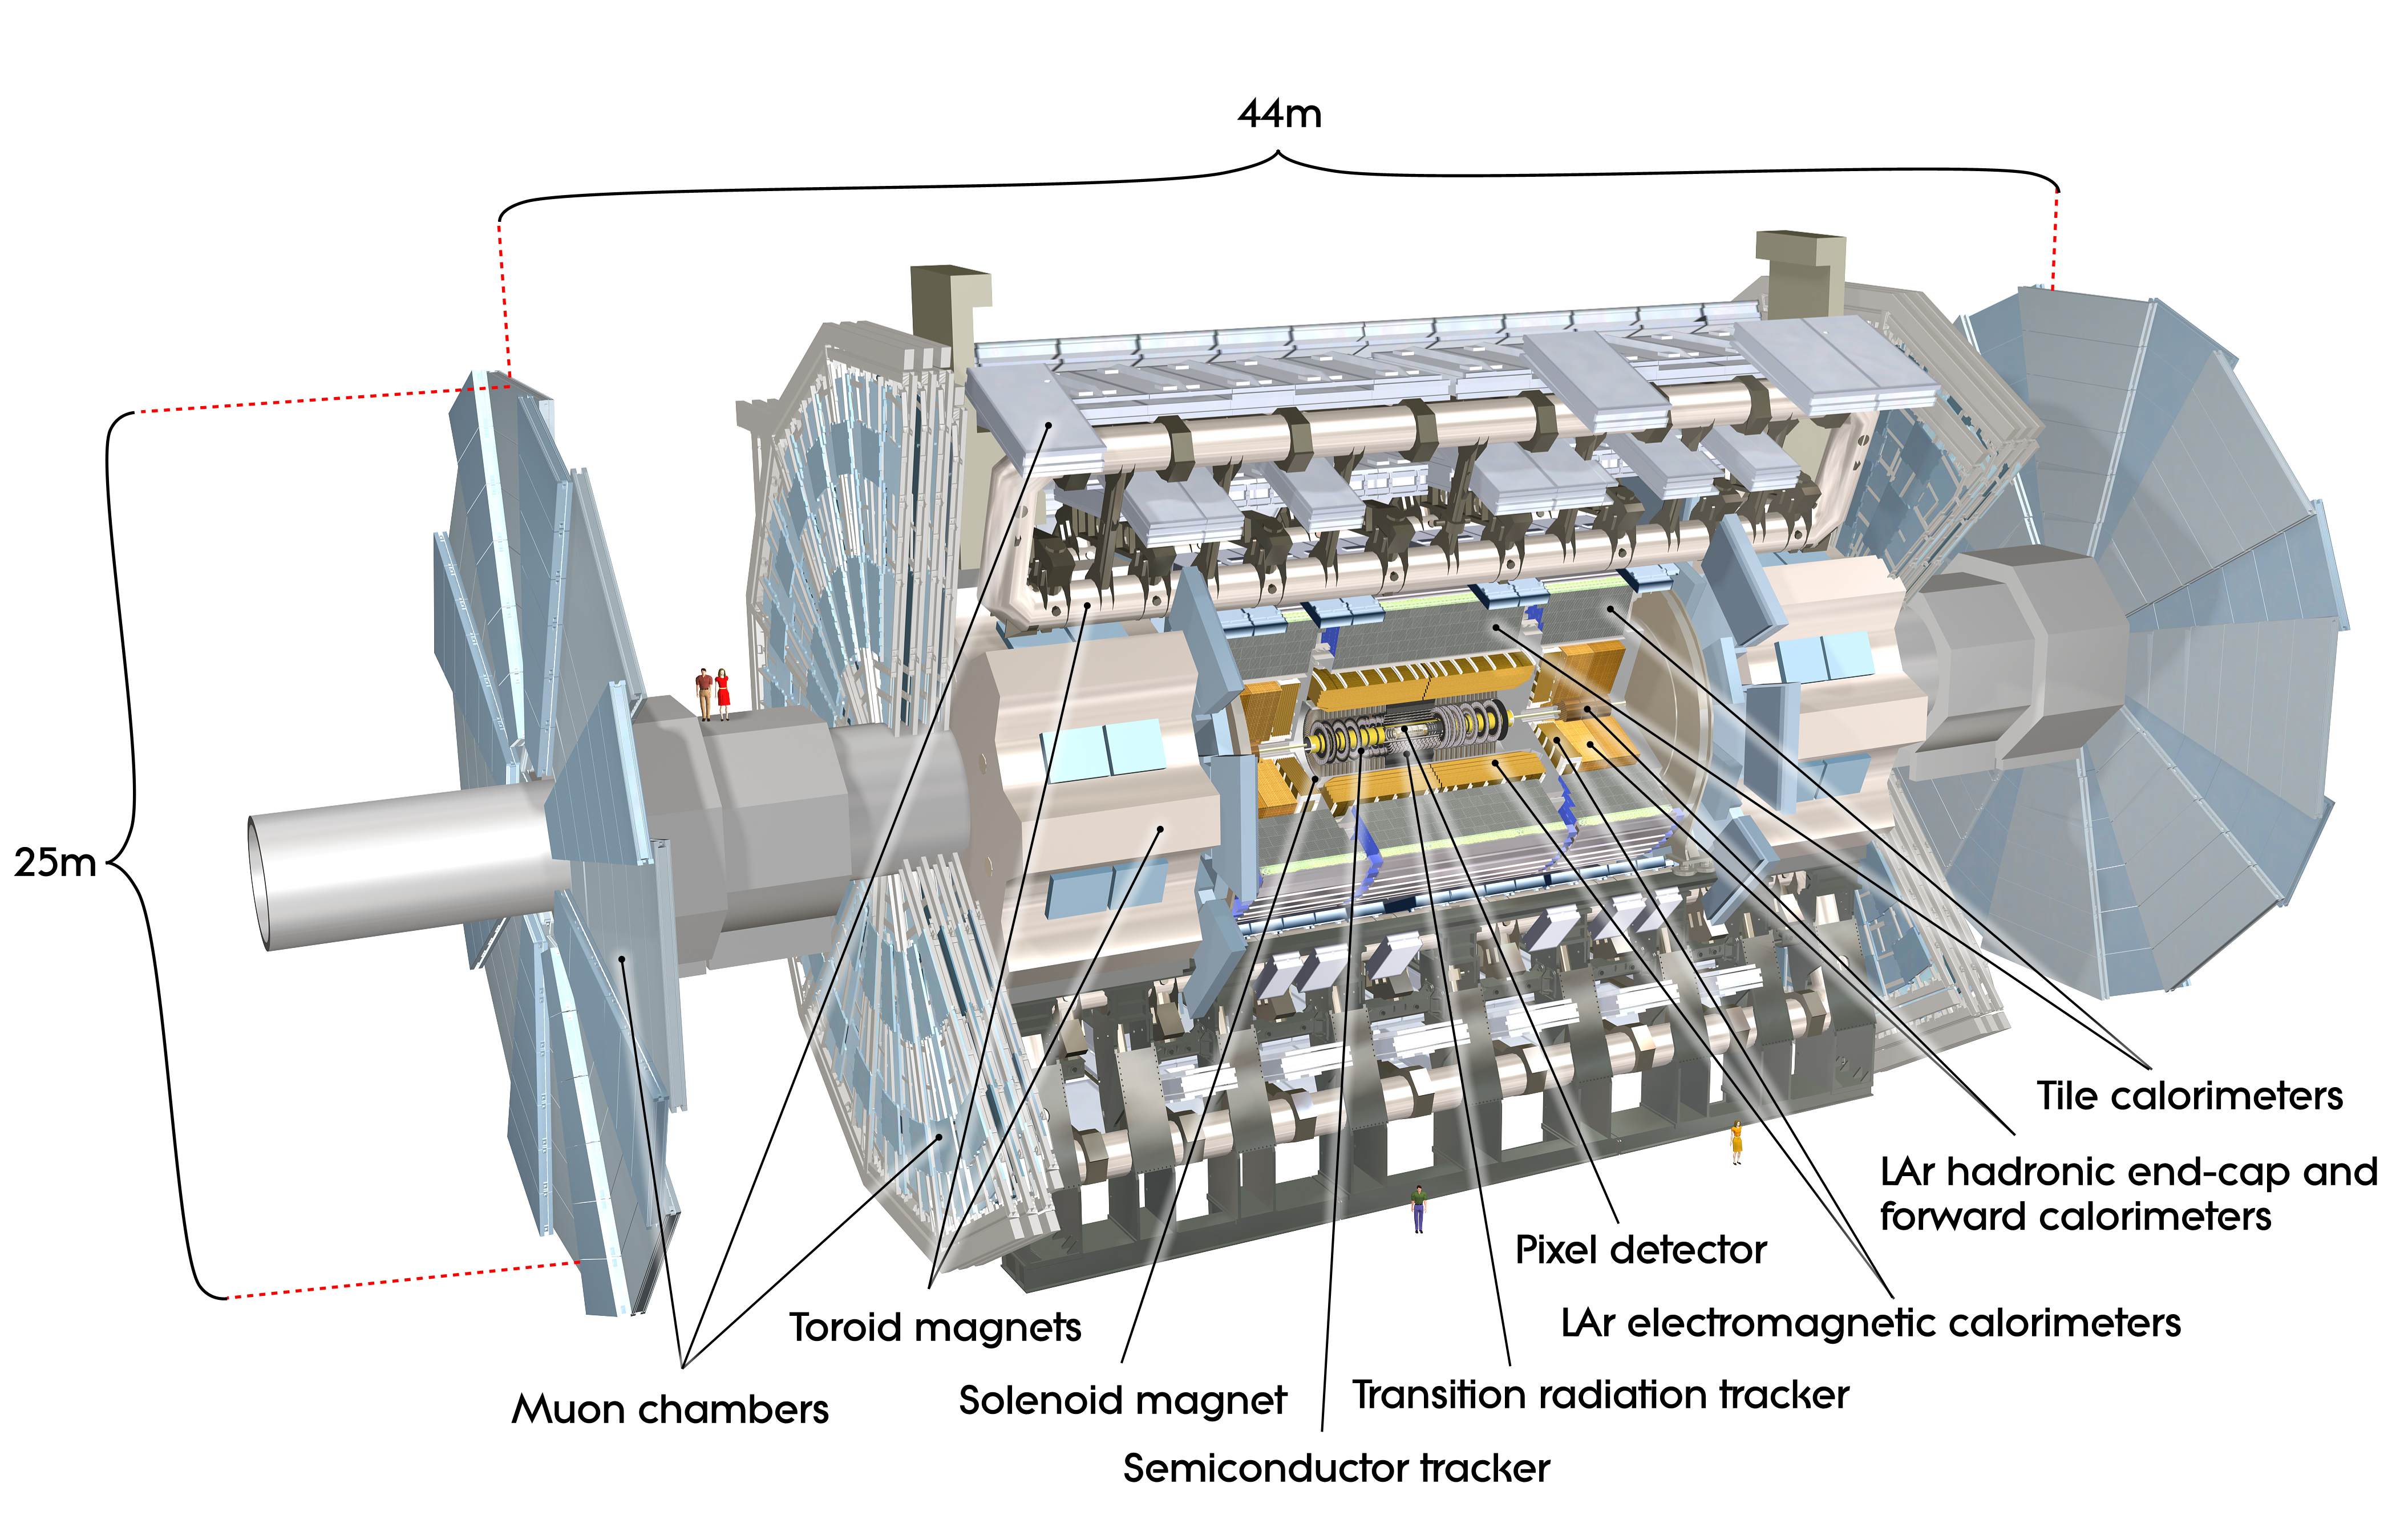
\includegraphics[clip,width=12cm]{fig/2/0803012_01.jpg}
  \caption{ATLAS検出器の全体図\cite{Aad:1129811}。直径 25 m、長さ 44 m の円筒型で、内部飛跡検出器、カロリーメータ、ミューオン検出器などの検出器を組み合わせて様々な粒子の測定を行っている。}
  \label{fig:2-4}
\end{figure}

\subsection{ATLAS検出器における座標系}\label{section2-2-1}
検出器の座標系を~\ref{fig:2-5}に示す。
ATLAS実験では直行座標系と円筒座標系が使用されており、直行座標系では、検出器の中心を原点として、ビーム軸に沿って$z$軸を取る。ビーム軸に垂直な平面を$x-y$平面としたときに、加速器の中心方向を正とする$x$軸及び、地面に対して垂直方向上向きを正とする$y$軸を設定する。円筒座標系では、ビーム軸に沿った$z$軸に対し、動径方向を$R$、ビーム軸周りの角度を方位角$\phi$、ビーム軸からの角度を極角$\theta$としている。
ATLAS検出器ではz軸が正の側をA-side、負の側をC-sideと定義している。

また、ATLAS実験で使用される座標系として、
\begin{equation}
 \eta=-\ln\bigg(\tan\frac{\theta}{2}\bigg)
 \label{ラピディティ}
\end{equation}
と定義される擬ラピディティ$\eta$が用いられる。
ATLAS 検出器は円筒形をしており、$|\eta| < 1.05$ の側面部分をバレル領域、$|\eta| > 1.05$ の底面部分をエンドキャップ領域と呼ぶ。

\begin{figure}[tb]
  \centering
  \includegraphics[clip, width=11cm]{fig/2/atlas_coordinate_fix.pdf}
  \caption{ATLAS検出器における座標系。}
  \label{fig:2-5}
\end{figure}

\newpage
\subsection{マグネットシステム}\label{section2-2-2}
ATLAS実験では、超電導磁石を用いて磁場をかけることにより荷電粒子の飛跡を曲げ、その曲率を図ることで横方向運動量を測定している。超電導磁石は2種類設置されており、衝突点付近で発生した荷電粒子の運動量測定のために用いられるソレノイド磁石と、ミューオンの運動量測定のために用いられるトロイド磁石である。ATLAS検出器の磁石の配置を図~\ref{fig:2-6}に示す。

\begin{figure}[tb]
  \centering
  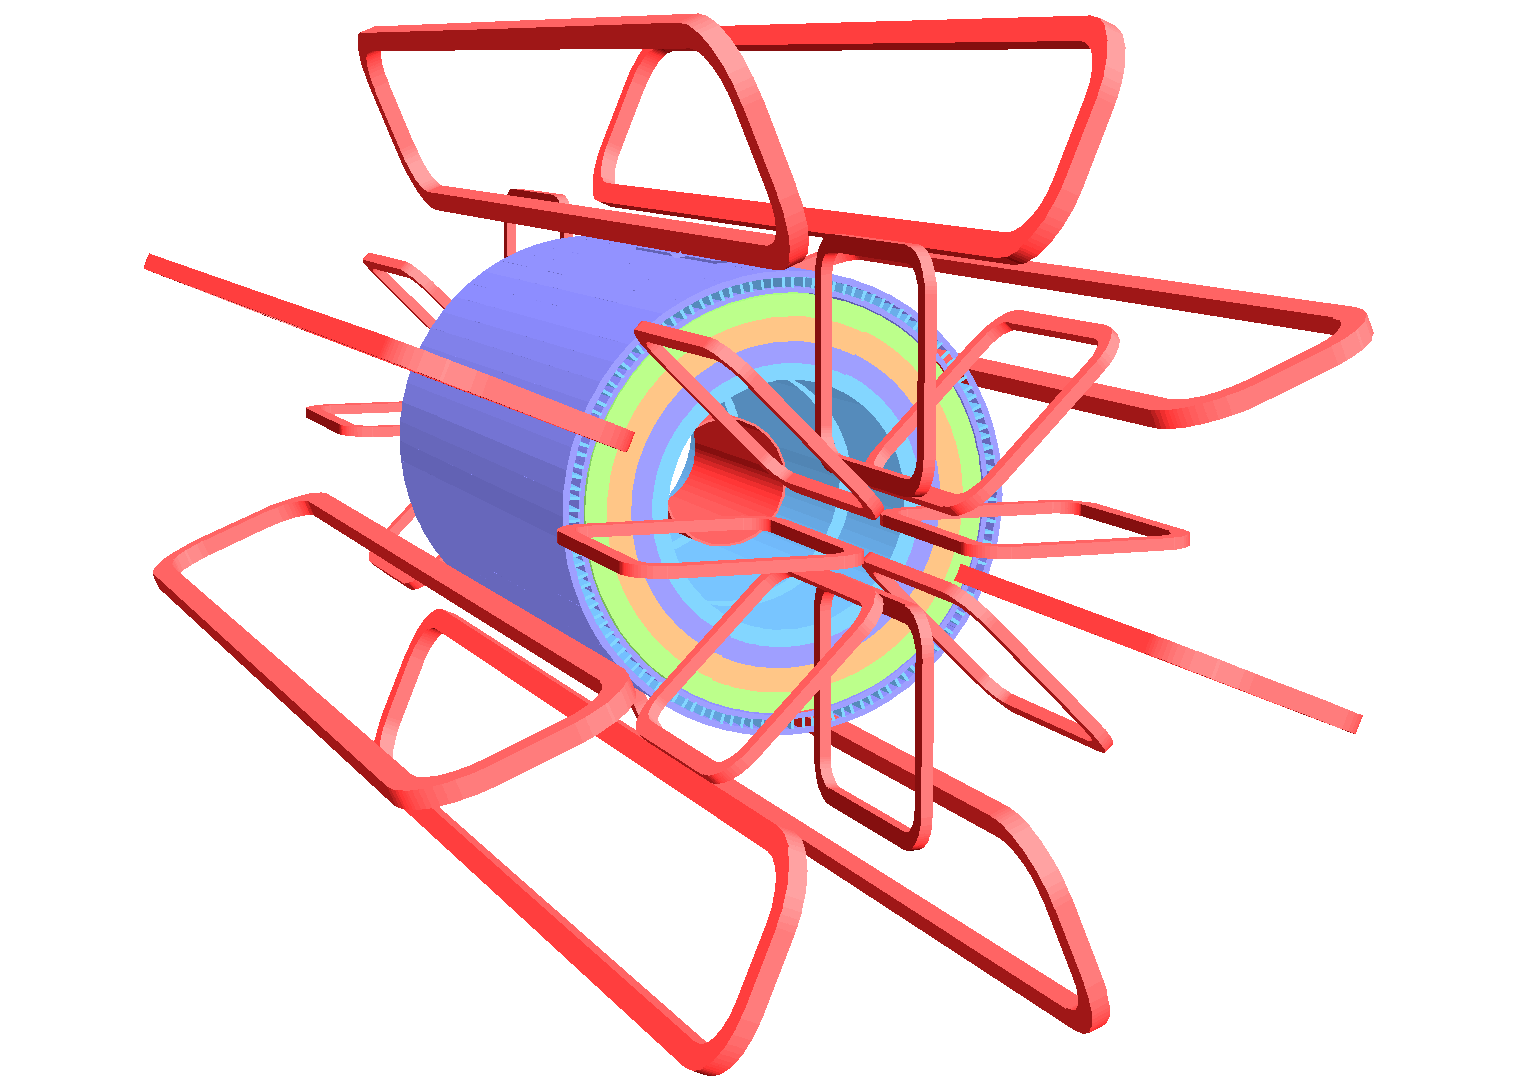
\includegraphics[clip, width=11cm]{fig/2/ATLcoilGeom.pdf}
  \caption{ATLAS検出器における超電導磁石の配置。}
  \label{fig:2-6}
\end{figure}

その全体は半径22m、全長26mである。
ソレノイド磁石は内部検出器とカロリーメータの間に設置されており、内径2.46m、外径2.56m、z軸方向の長さ5.8mの円筒形である。内部に2Tの磁場をかけており、内部検出器中で荷電粒子の飛跡を$\phi$方向に曲げて横運動量の測定を行う。
また、トロイド磁石はカロリメータの外側に設置されており、1つのバレルトロイドとA-side、C-side両側にそれぞれ1つずつ設置されているエンドキャップトロイドで構成され、それらがビーム軸に対して8回対称になるように配置されている。バレルトロイドは内径9.4m、外径20.1m、z軸方向の長さ25.3mで、エンドキャップトロイドは内径1.65m、外径10.7m、z軸方向の長さ5.0mである。
また磁場の強さはそれぞれ、バレルトロイドでは約0.5T、エンドキャップトロイドでは約1Tである。
トロイド磁石によって生じる磁場の$\eta$分布と$x-y$平面での磁場の分布をそれぞれ図~\ref{fig:2-7-1}、図~\ref{fig:2-7-2}で示す。

\begin{figure}[h]
  \begin{minipage}[b]{0.45\linewidth}
      \centering
      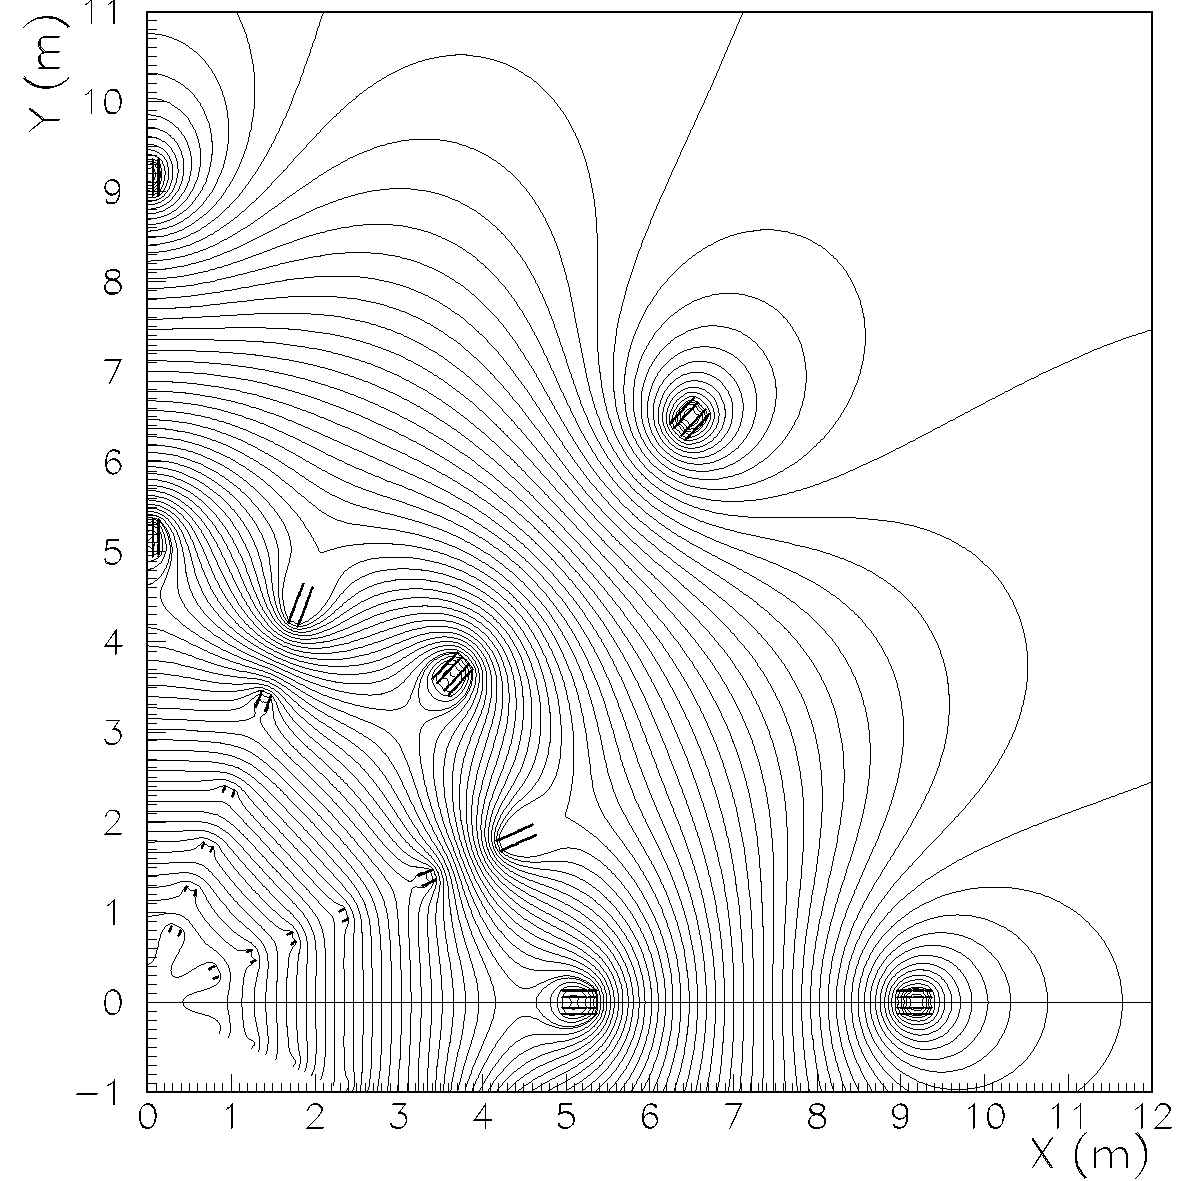
\includegraphics[clip, width=5cm]{fig/2/FMBmap.pdf}
      \subcaption{トロイド磁石による磁場の$\phi$分布。}
      \label{fig:2-7-1}
  \end{minipage}
    \begin{minipage}[b]{0.48\linewidth}
      \centering
      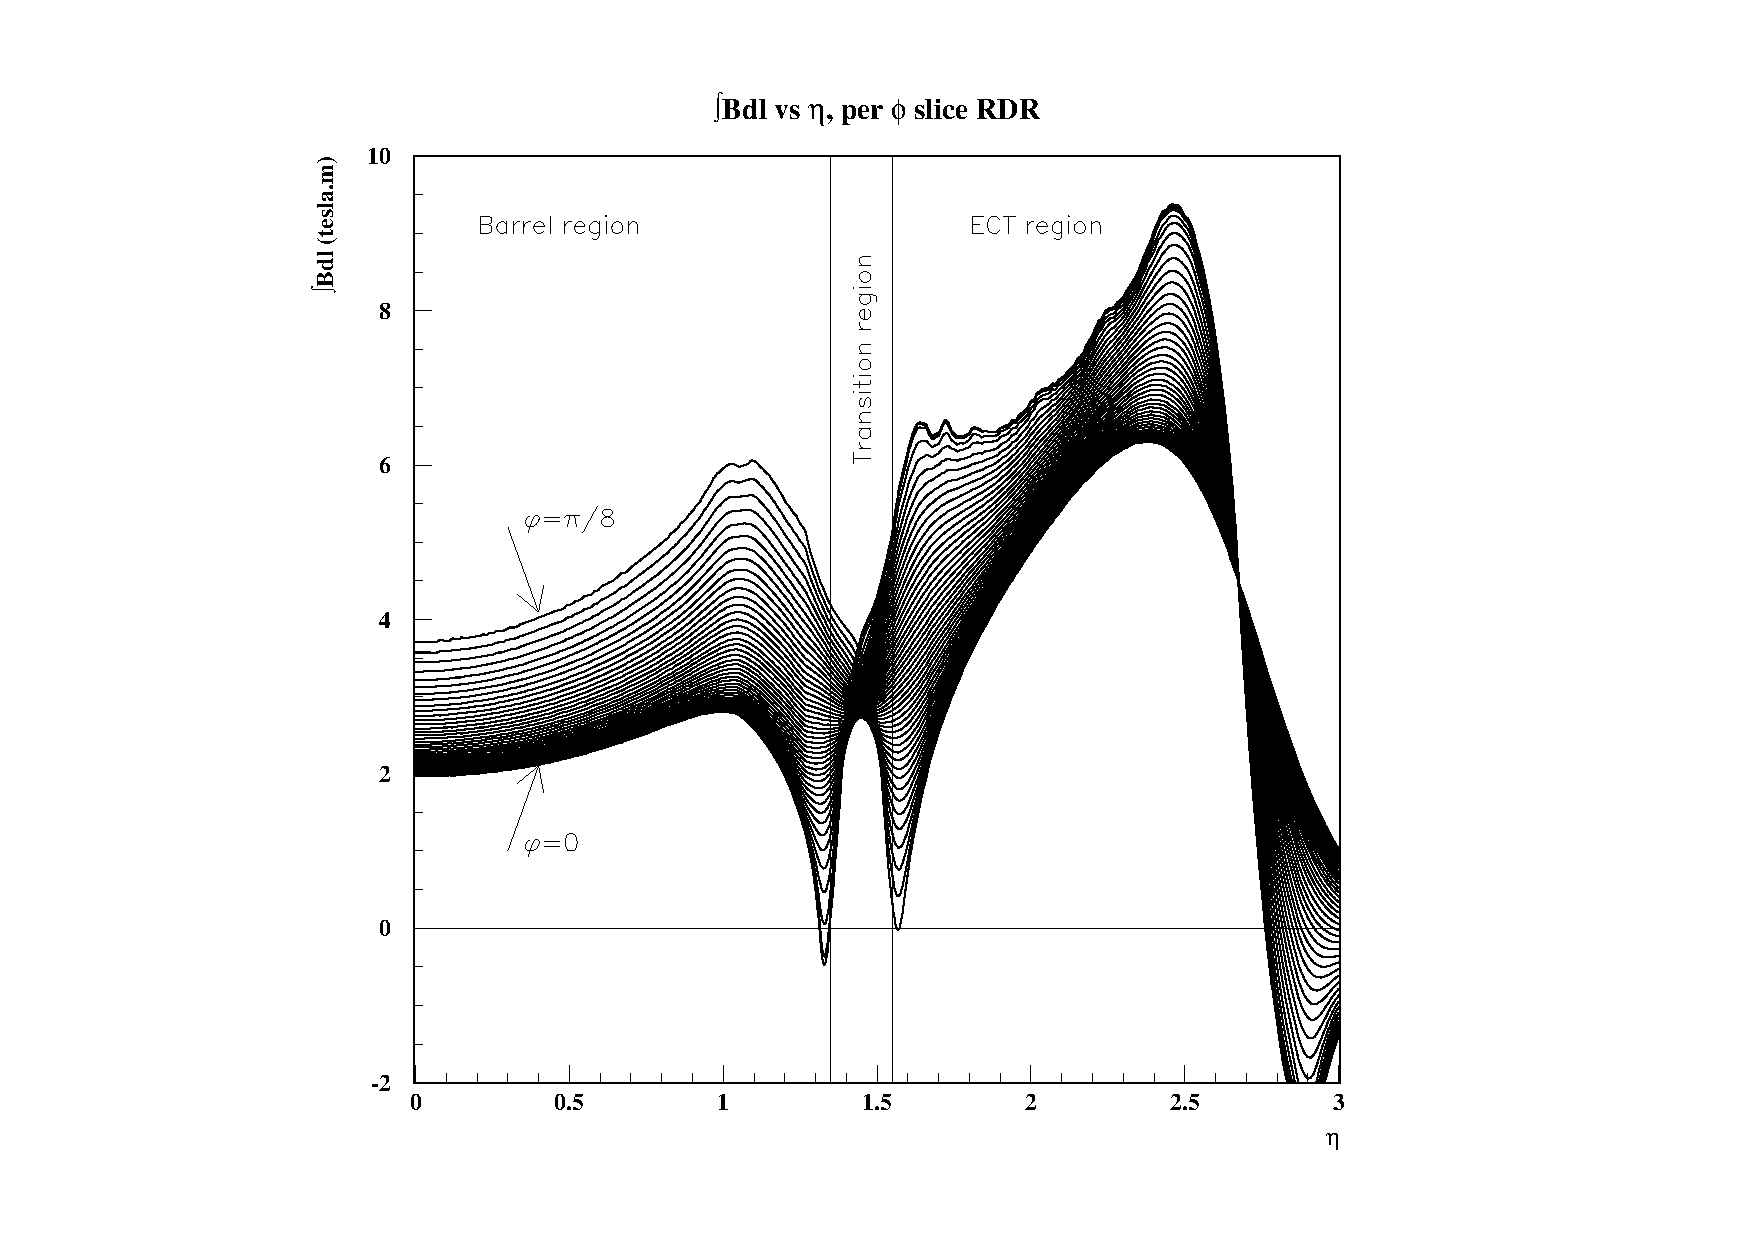
\includegraphics[clip, width=8cm]{fig/2/bdl.pdf}
      \subcaption{ビーム軸に垂直な$x-y$平面での磁場の分布。}
      \label{fig:2-7-2}
  \end{minipage}
  \caption{超電導磁石による磁場分布\cite{article:ATLASMagneticField}。}
\end{figure}

\subsection{内部飛跡検出器}\label{2-2-3}
内部飛跡検出器は内側からInsertable~B~Layer~(IBL)、Pixel検出器、SemiConductor~Tracker~(SCT)、Transition~Radiation~Tracker~(TRT)で構成される。バレル領域とエンドキャップ領域における内部飛跡検出器の配置をそれぞれ図~\ref{fig:2-8-1}、図~\ref{fig:2-8-2}に示す。
内部飛跡検出器は半径約1.1m、z軸方向に長さ約5.3mで、$|\eta|<2.5$の領域を覆っている。
検出器内には、前述のとおりソレノイド磁石によって約2Tの磁場がかかっており磁場領域を通過した荷電粒子の飛跡の$\theta$方向の曲率から運動量を計算する。

\begin{figure}[h]
  \begin{minipage}[b]{0.5\linewidth}
      \centering
      \includegraphics[clip, width=6cm]{fig/2/inner_detector2.jpg}
      \subcaption{バレル領域}
      \label{fig:2-8-1}
  \end{minipage}
    \begin{minipage}[b]{0.5\linewidth}
      \centering
      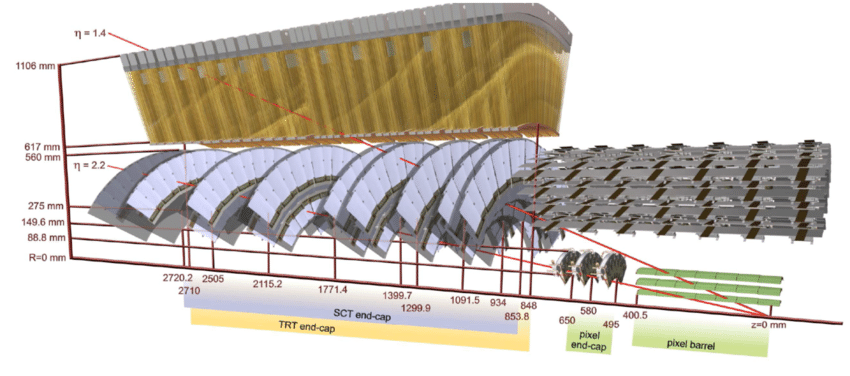
\includegraphics[clip, width=8cm]{fig/2/inner_detector3.png}
      \subcaption{エンドキャップ領域}
      \label{fig:2-8-2}
  \end{minipage}
  \caption{バレル領域とエンドキャップ領域での内部飛跡検出器の構造\cite{Aad:1129811}。}
\end{figure}

\subsubsection{Pixel検出器とIBL}
Pixel検出器はバレル領域で同心円状に3層、エンドキャップ両飯豊A-side、C-side両側にそれぞれディスク状に3層設置されている。1つのpixelサイズは50$\mu$m$\times$ 400$\mu$mであり、R$\phi$方向及び$z$方向に並べて配置している。
pixel検出器の位置分解能は、R$\phi$方向に10$\mu$m、$z$方向に115$\mu$mである。

また、Run-2からルミノシティ増加への対応とPixel検出器の性能向上のためにPixel検出器よりも内側に配置された。1つのpixelのサイズは50$\mu$m$\times$ 250$\mu$mであり、位置分解能はR$\phi$方向に10$\mu$m、$z$方向に75$\mu$mである。IBLにより、衝突点と飛跡の距離であるImpact Parameterの測定精度が改善された。

\begin{figure}[h]
  \centering
  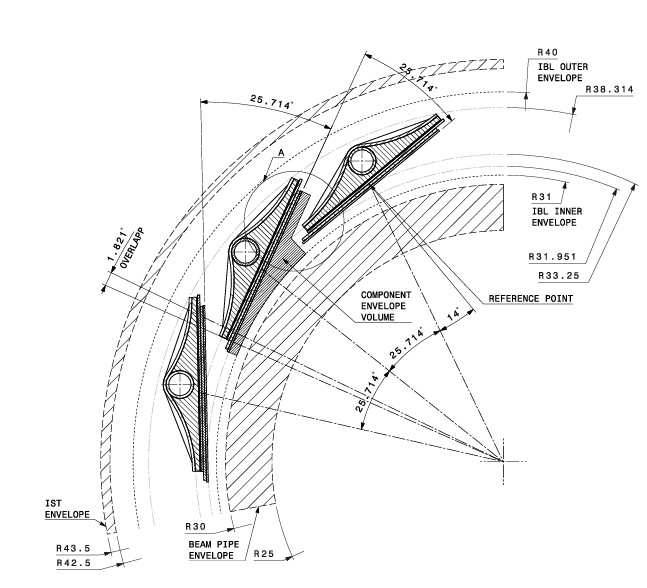
\includegraphics[clip, width=9.5cm]{fig/2/IBL_layout.png}
  \caption{IBLのレイアウト~\cite{article:ATLASBlayerTDR}。}
  \label{fig:2-9}
\end{figure}

\subsubsection{SCT}
SCTはバレル領域で4層からなる同心円状のシリンダ形状で設置されており、エンドキャップ領域でA-side、C-sideそれぞれ9枚ずつのディスク形状になっている。
SCTの位置分解能はバレル領域でR方向に17$/mu$m、$\phi$方向に580$\mu$m、エンドキャップ領域ではR方向に17$\mu$m、$z$方向に580$\mu$mである。


\subsubsection{TRT}
TRTはドリフトチューブを積み重ねるように構成されており、$|\eta|<2.0$の領域を覆っている。バレル領域では長さ144cmのチューブをビーム軸と平行に、エンドキャップ領域では長さ37cmのチューブを放射状に配置している。TRTの位置分解能はR-$\phi$方向に130$\mu$mである。

また、TRTでは荷電粒子が誘電率の異なる物質へ入社する際に光子を放出する「遷移放射」を利用した電子の同定も行っている。遷移放射で放出される光子のエネルギーは粒子のローレンツ因子$\gamma$に比例するため、これを利用することで入射した荷電粒子が電子かどうか判定している。

\subsection{カロリメータ}\label{2-2-4}
カロリメータは内部飛跡検出器の外側に設置されており、内側から電磁カロリメータ、ハドロンカロリメータの順に配置されている。電磁カロリメータは電磁相互作用による電磁シャワーを用いて電子と光子のエネルギーを測定し、ハドロンカロリメータは強い相互作用によるハドロンシャワーを用いてハドロンのエネルギー測定やそれを組み合わせたジェット再構成に用いられる。ATLAS検出器におけるカロリメータの概要図を図~\ref{fig:2-10}に示す

\begin{figure}[h]
  \centering
  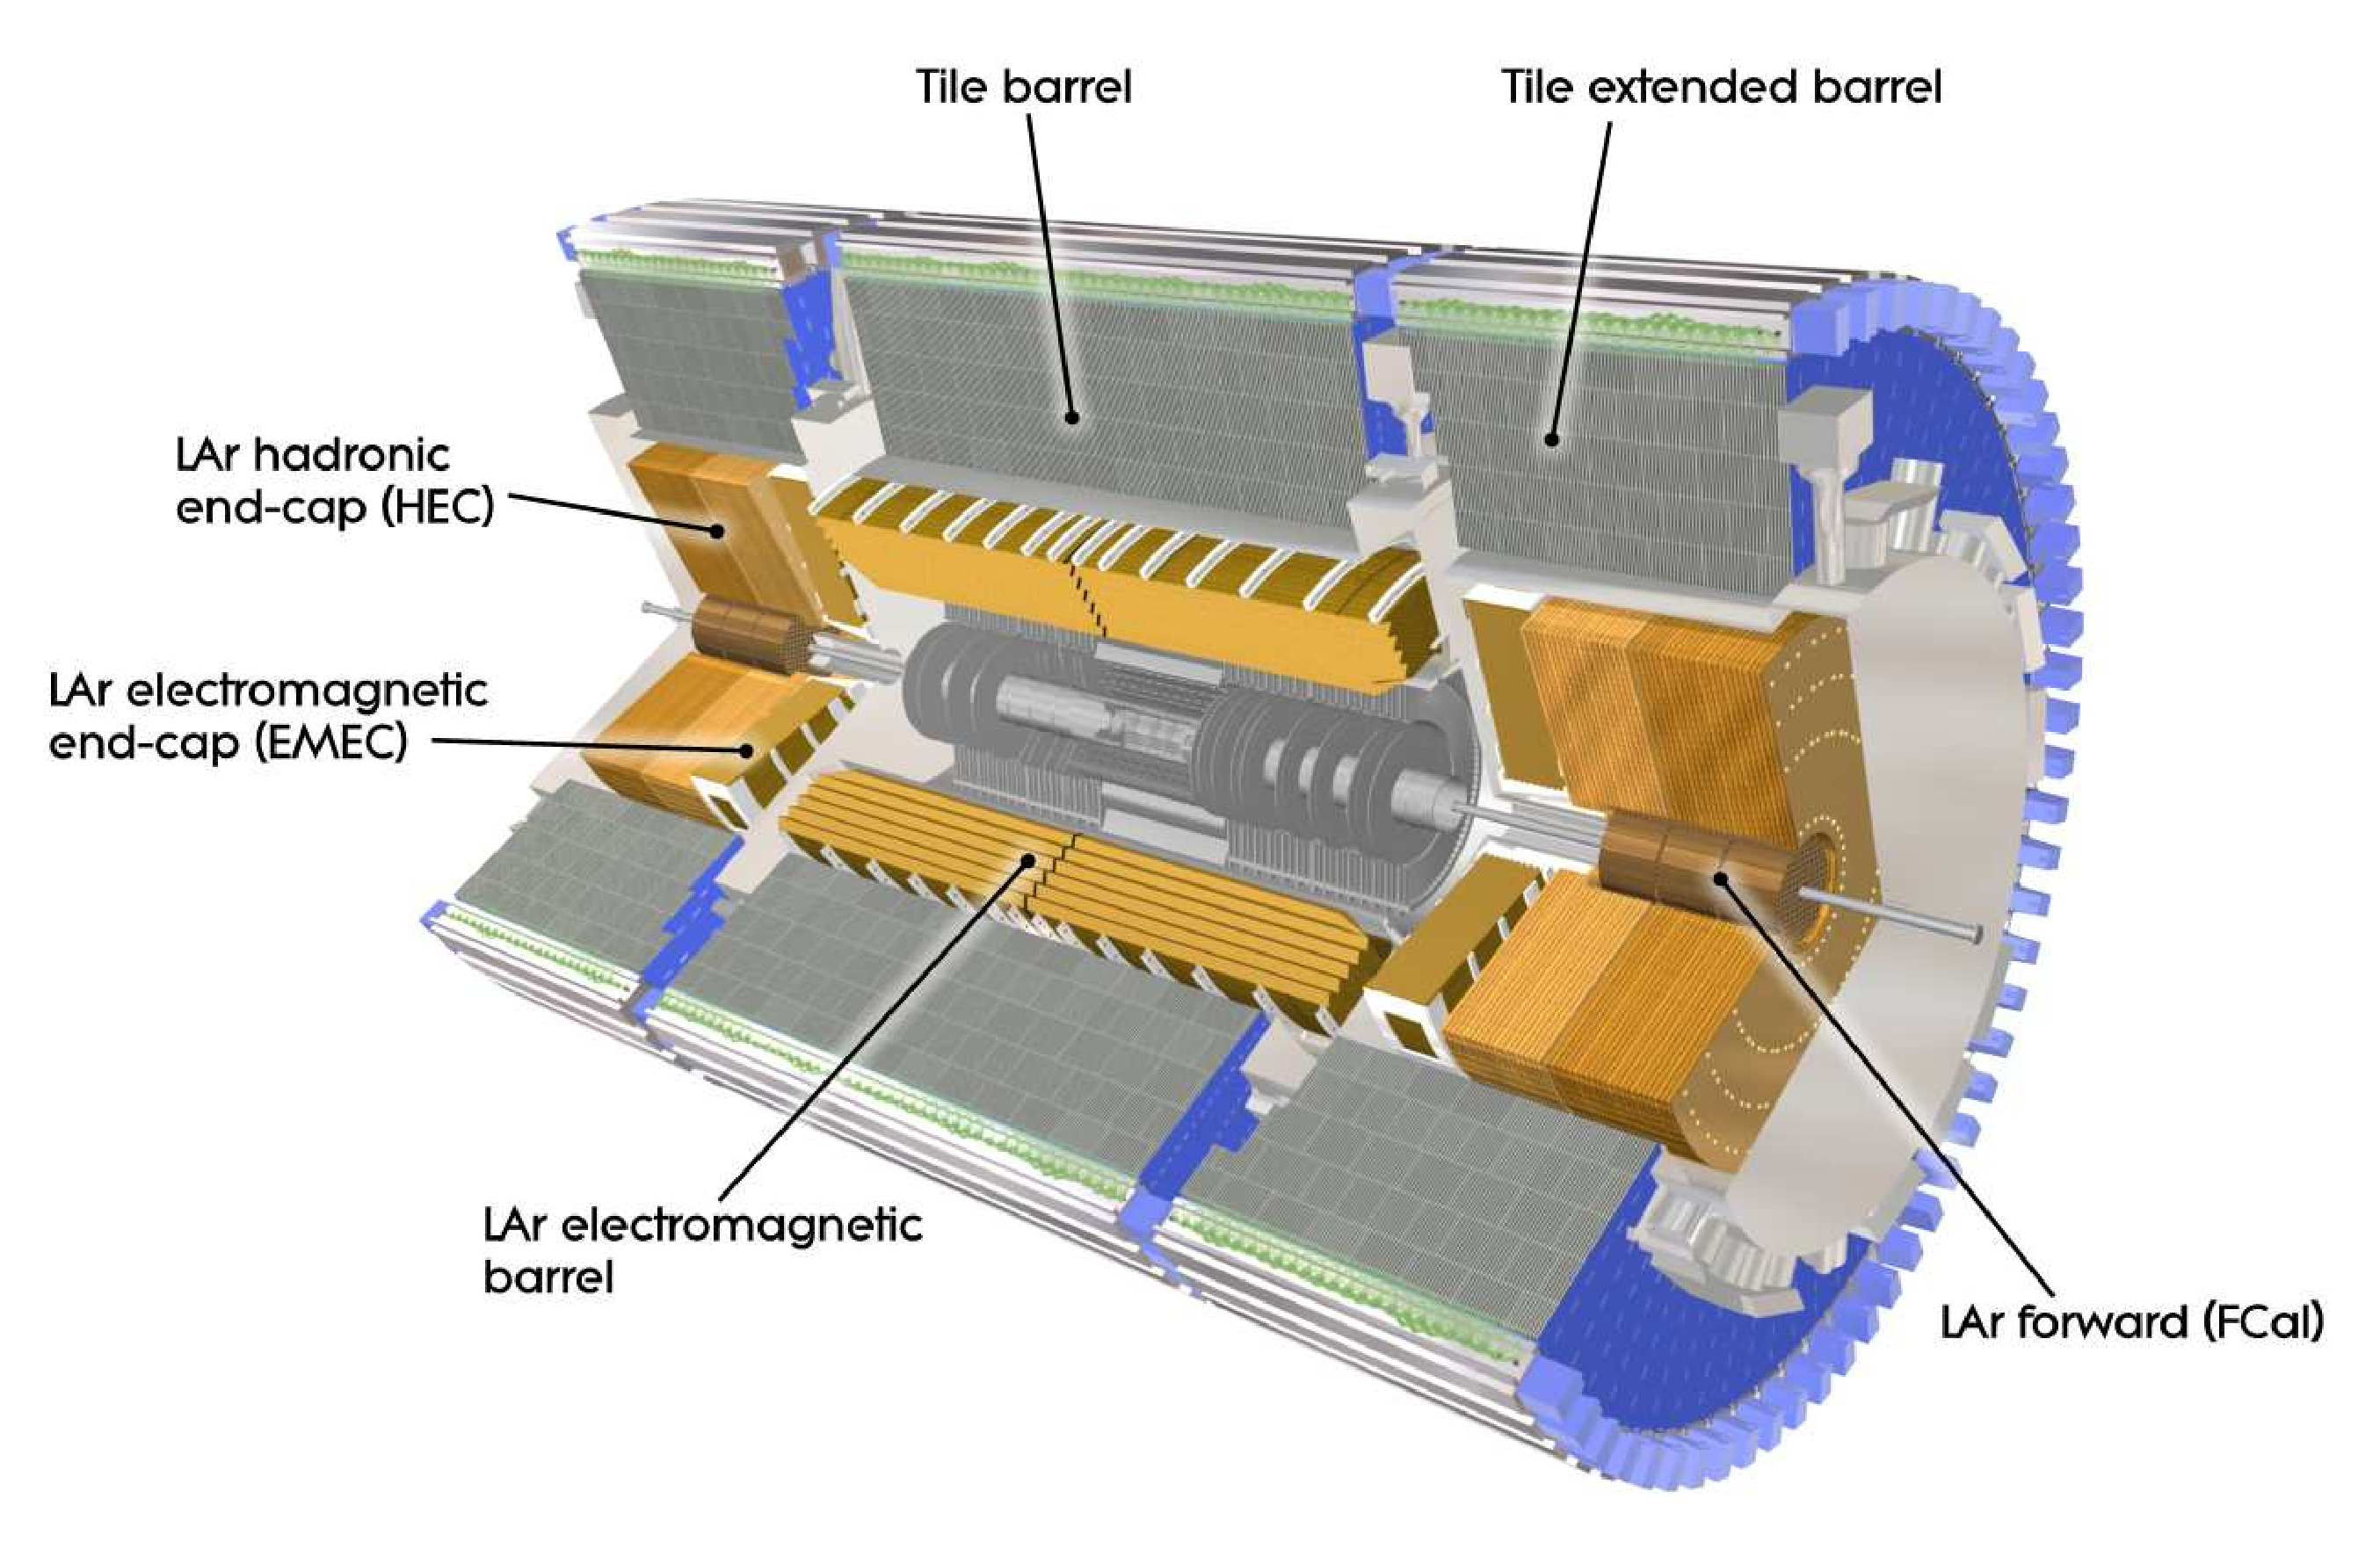
\includegraphics[clip, width=9cm]{fig/2/Calorimeter_d3.pdf}
  \caption{カロリメータの全体図~\cite{Aad:1129811}。}
  \label{fig:2-10}
\end{figure}

\subsubsection{電磁カロリメータ}
電磁カロリメータはバレル領域をカバーするように$|\eta|<1.5$にバレル電磁カロリメータ、エンドキャップ領域をカバーするように$1.4<|\eta|<3.2$にエンドキャップ電磁カロリメータが配置されている。
それぞれの厚さは、バレル領域で放射長の22倍以上、エンドキャップ領域で放射長の24倍以上である。
電磁カロリメータは$\phi$方向の不感領域を失くすために鉛の吸収体と強い放射線耐性を持つ液体アルゴンをアコーディオン状に組み合わせた構造になっている(~\ref{fig:2-11})。


\begin{figure}[h]
  \centering
  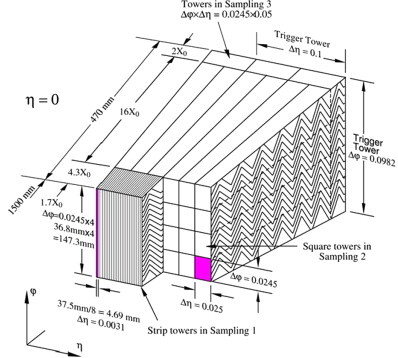
\includegraphics[clip, width=9cm]{fig/2/electoricCal.jpg}
  \caption{電磁カロリメータの構造~\cite{Aad:1129811}。}
  \label{fig:2-11}
\end{figure}

\subsubsection{ハドロンカロリメータ}
ハドロンカロリメータは、電磁カロリメータと同様にバレル領域をカバーするために$|\eta|<1.7$とエンドキャップ領域をカバーするために$1.5<|\eta|<3.2$に配置されている。
バレル領域では、鉄の吸収体とシンチレータを交互に重ねたTileカロリメータ(図~\ref{fig:2-12-1})が設置されている。シンチレーション光を波長変換ファイバーで集め、光電子増倍管で読み出しを行っている。
エンドキャップ領域では、銅の吸収体と液体アルゴンから構成されたハドロンエンドキャップカロリメータ(図~\ref{fig:2-12-2})が使用されている。
バレル領域とエンドキャップ領域に加えて、$3.1<|\eta|<4.9$のフォワード領域をカバーするために銅とタングステンの吸収体と液体アルゴンから構成されたフォワードカロリメータが設置されている。

\begin{figure}[h]
  \begin{minipage}[b]{0.5\linewidth}
      \centering
      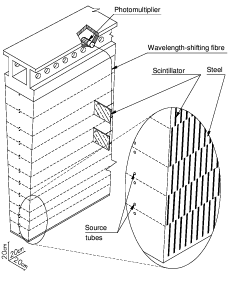
\includegraphics[clip, width=6cm]{fig/2/TileCalo.png}
      \subcaption{Tileカロリメータ}
      \label{fig:2-12-1}
  \end{minipage}
    \begin{minipage}[b]{0.5\linewidth}
      \centering
      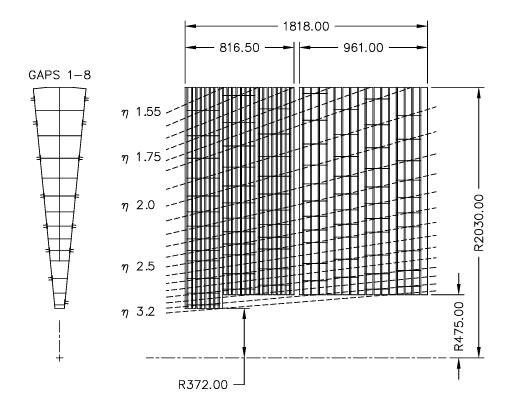
\includegraphics[clip, width=8cm]{fig/2/HadronEndcapCal.png}
      \subcaption{エンドキャップ領域におけるカロリメータ}
      \label{fig:2-12-2}
  \end{minipage}
  \caption{バレル領域とエンドキャップ領域でのハドロンカロリメータの構造\cite{Aad:1129811}。}
\end{figure}


\subsection{ミューオン検出器}\label{section2-2-5}
ミューオン検出器はATLAS検出器の一番外側に配置されており、カロリメータから出てきた荷電粒子の位置や横方向運動量を測定する。トリガー用の検出器として~Resistive~Plate~Chamber~(RPC)とThin~Gap~Chamber~(TGC)、精密測定用の検出器として~Monitored~Drift~Tube~(MDT)の3つの検出器で構成される。またRun-3からエンドキャップ領域の磁場領域より内側に設置されていた~Small~Wheelに代わって~New~Small~Whell~(NSW)という検出器が導入された。
図~\ref{fig:2-13}にミューオン検出器の全体図を示す。

\begin{figure}[h]
  \centering
  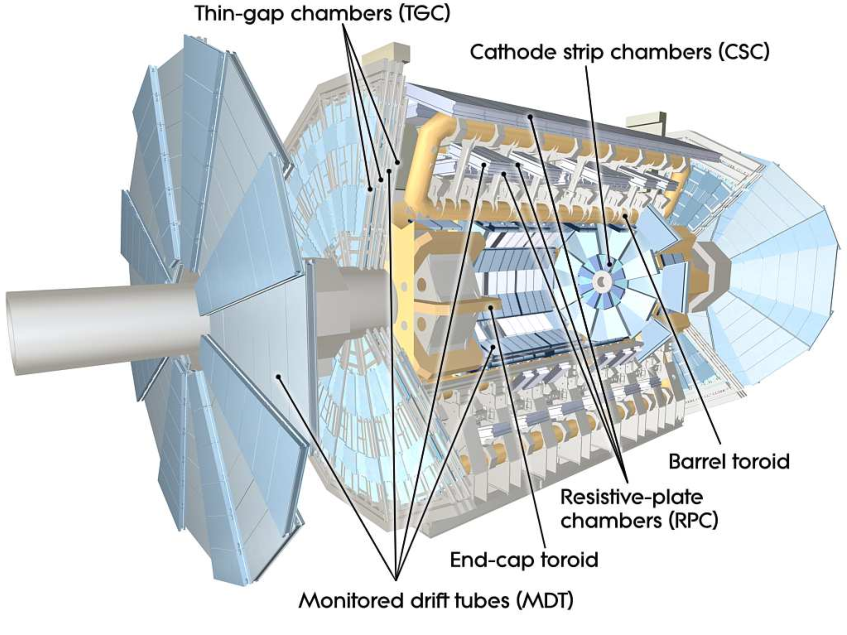
\includegraphics[clip, width=9cm]{fig/2/muondetector.pdf}
  \caption{ミューオン検出器の全体図~\cite{Aad:1129811}。バレル領域にRPC、MDT、エンドキャップ領域にTGC、MDTが配置されている。}
  \label{fig:2-13}
\end{figure}

ミューオン検出器では、各検出器をステーションと呼ばれる層状にまとめられている。これらのステーションはバレル領域とエンドキャップ領域でそれぞれ3層あり、衝突点に近い方からインナーステーション~(I)、ミドルステーション~(M)、アウターステーション~(O)と呼ばれる。バレル領域ではビーム軸周りに半径約5m、7m、10mのところに同心円状にステーションが並べられ円筒状の検出器を形成している。
エンドキャップ領域では、$|z|$が約7.4m、14m、21.5mの位置に$z$軸に垂直にステーションが配置されており大きなホイールを形成している。また、インナーステーションとミドルステーションの間に~Endcap~Extra~(EE)と呼ばれる検出器が設置されている。

また、図~\ref{fig:2-14}で示されているように、ミューオン検出器は不感領域を失くすために$\phi$方向に大きさの違う2つのセクターを互い違いに8つずつ$\phi$方向に重ねられている。衝突点に近い方から、~Small~sectorと~Large~sectorと呼ばれる。
ミューオン検出器の~Large~sector、~Small~sectorの$R-z$平面の断面図を図~\ref{fig:2-15-1}、図~\ref{fig:2-15-2}に示す。

\begin{figure}[h]
  \centering
  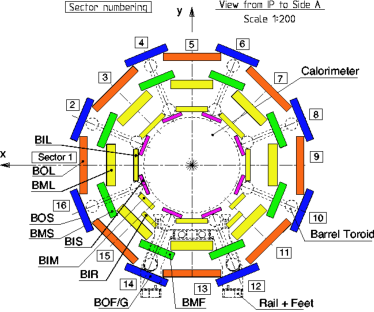
\includegraphics[clip, width=8cm]{fig/2/muon_detector_xy.pdf}
  \caption{ミューオン検出器の$x-y$平面での断面図~\cite{Aad:1129811}。黄と橙が~Small~sector、緑と青が~Large~sector。}
  \label{fig:2-14}
\end{figure}

%-------------チェンバーの略称と検出器の対応表を書く------------------------------

\begin{figure}[h]
  \begin{minipage}[b]{0.5\linewidth}
      \centering
      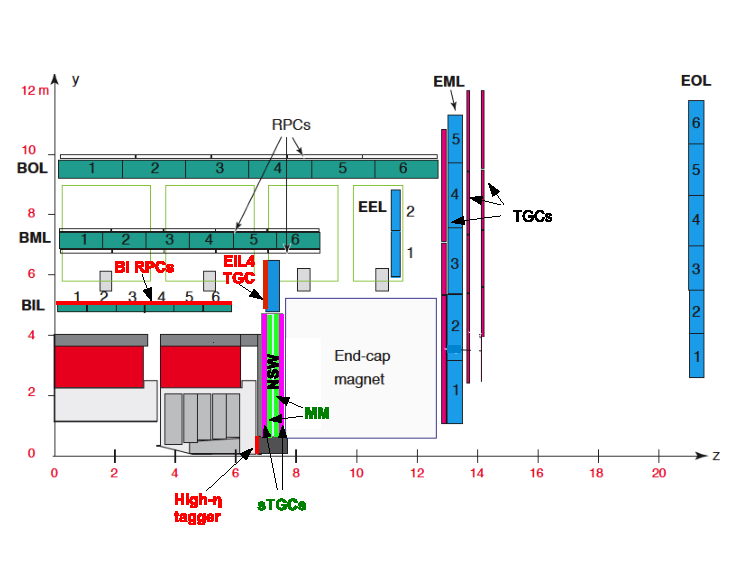
\includegraphics[clip, width=8cm]{fig/2/muon_Rz_Large.pdf}
      \subcaption{Large~sector}
      \label{fig:2-15-1}
  \end{minipage}
    \begin{minipage}[b]{0.5\linewidth}
      \centering
      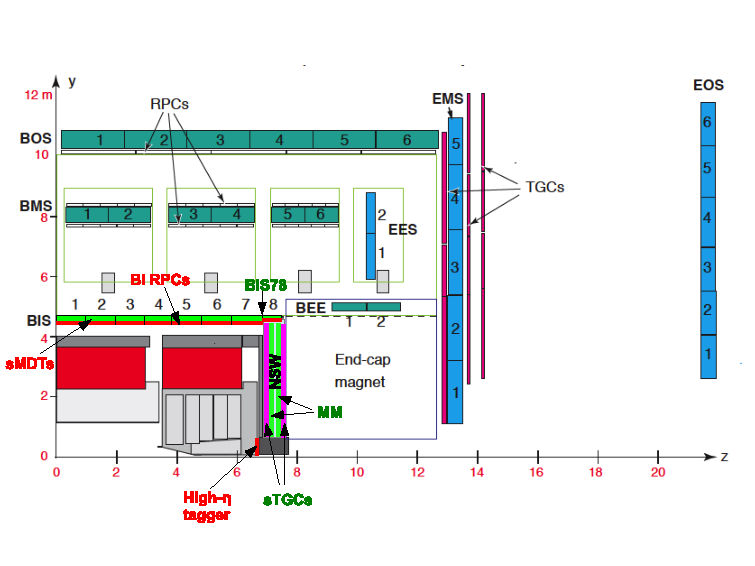
\includegraphics[clip, width=8cm]{fig/2/muon_Rz_small.pdf}
      \subcaption{Small~sector}
      \label{fig:2-15-2}
  \end{minipage}
  \caption{ミューオン検出器の~Large~sector、~Small~sectorの$R-z$平面の断面図\cite{article:phase2}。}
\end{figure}

\subsubsection{Resisitive Plate Chamber (RPC)}
RPCはバレル領域に設置されている、主にミューオントリガー用のガス検出器である。
構造を図~\ref{fig:2-16}に示す。2枚の高抵抗プレートの間に幅~2mmの絶縁体が挟み込まれており、プレート間には約 ~4.9kV/mmの電場が形成されている。
プレート間には、$\rm{C_{2}H_{2}F_{4}/Iso - C_{4}H_{10}/SF_{6}(94.7 : 5 : 0.3)}$の混合ガスが充填されている。
ミューオンが通過した際に、ガスから電離した電子が電場に沿って雪崩増幅を起こし、プレートの外側に取り付けられたストリップで信号を読み出す。

\begin{figure}[h]
  \centering
  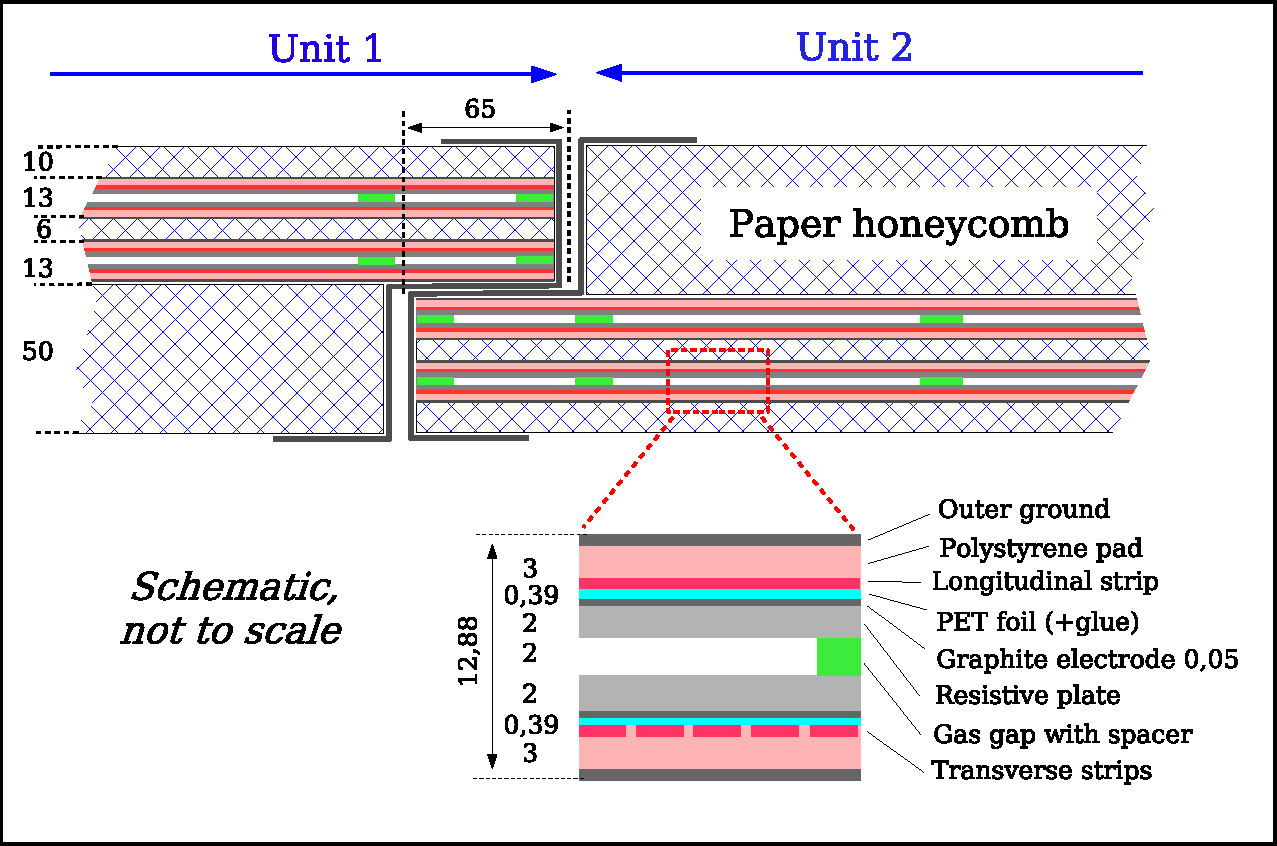
\includegraphics[clip, width=8cm]{fig/2/RPC_structure.pdf}
  \caption{RPC検出器の構造~\cite{Aad:1129811}。}
  \label{fig:2-16}
\end{figure}

図~\ref{fig:2-17}で表されるように、Large~sectorと~Small~sectorそれぞれに、MDTミドルステーションを挟み込むように2枚、MDTアウターステーションの外側に1枚の、計3枚のRPCが配置されている。
1枚のRPCは直交した$\eta$~-stripと$\phi$-~stripから構成されており、2次元での読み出しを行う。
MDTでは$\phi$方向の測定ができないので、RPCで測定した$\phi$の情報を用いる。

\begin{figure}[h]
  \centering
  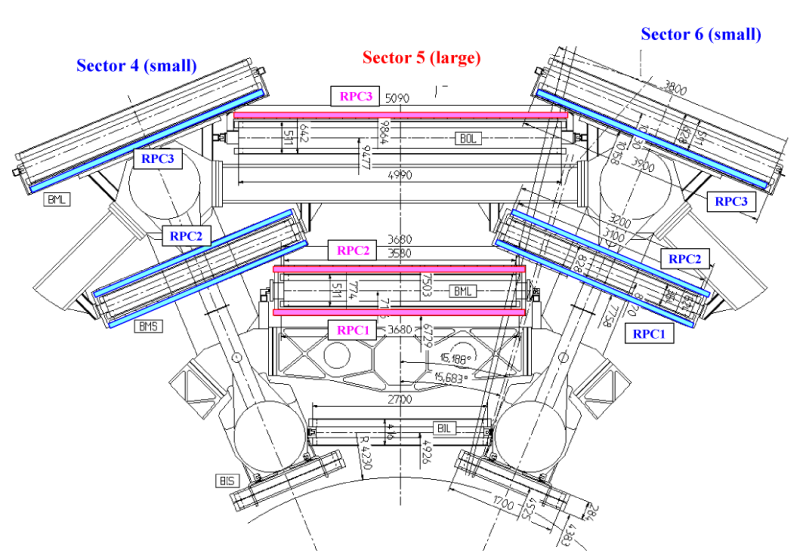
\includegraphics[clip, width=8cm]{fig/2/RPC_xy.pdf}
  \caption{RPC検出器の$x-y$平面での断面図~\cite{Aad:1129811}。}
  \label{fig:2-17}
\end{figure}

\subsubsection{Thin Gap Chambers (TGC)}
TGCはエンドキャップ領域に設置されている、主にミューオントリガー用のガス検出器である。
構造を図~\ref{fig:2-18}に示す。
TGCの各層は、ワイヤーとアノード層、ストリップ層から構成されているマルチワイヤーガス検出器で、$\eta$方向をワイヤー、$\phi$方向をストリップで測定している。内部には、$\rm{CO_{2}}$と$\rm{n - C_{5}H_{12}}$ガスが充填されている。
ワイヤー間の距離を1.8mm、ワイヤーとストリップの距離を1.4mmと短くすることによって高い時間分解能を実現している。

\begin{figure}[h]
  \centering
  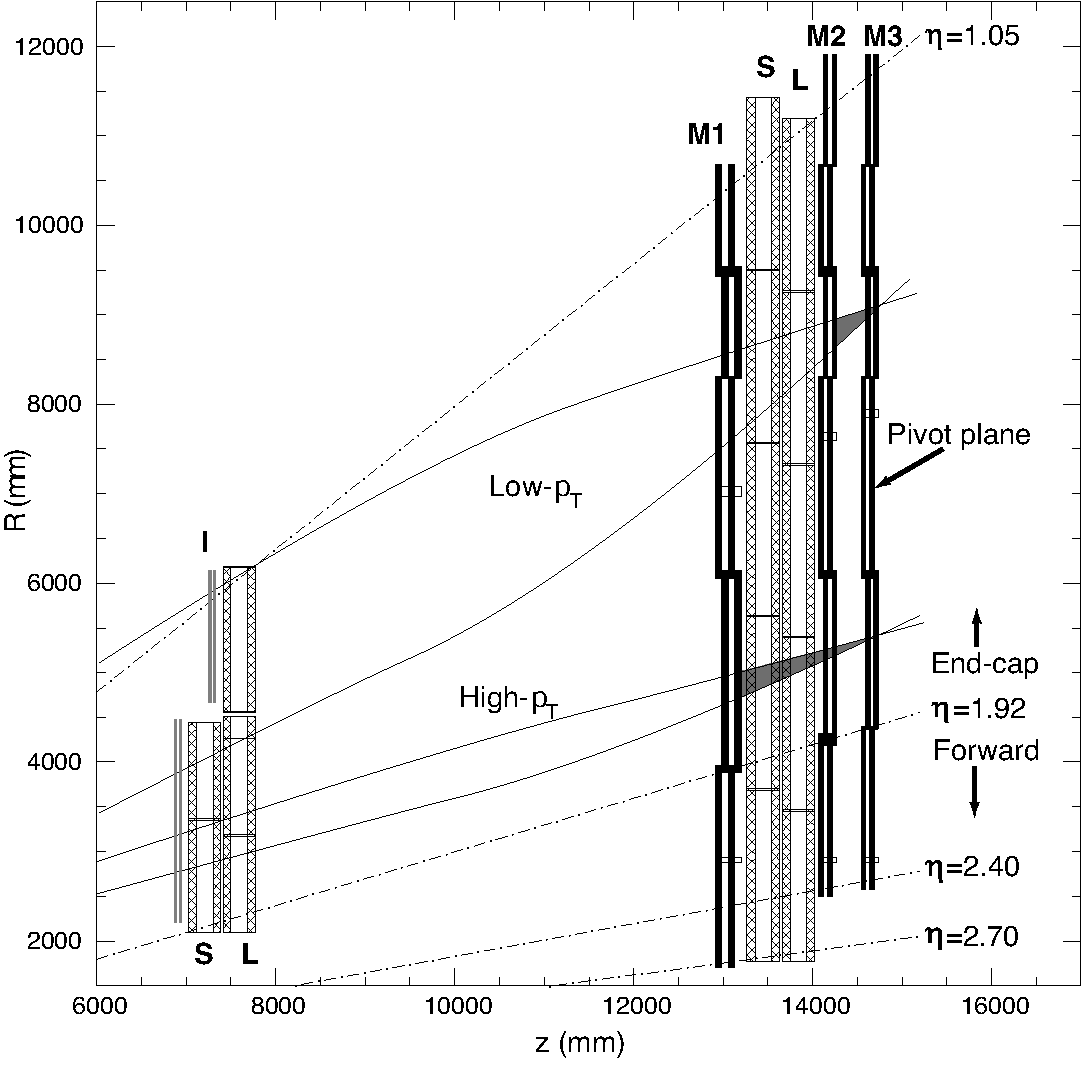
\includegraphics[clip, width=8cm]{fig/2/l1mue-schema.pdf}
  \caption{TGC検出器の配置~\cite{Aad:1129811}。}
  \label{fig:2-18}
\end{figure}

図~\ref{fig:2-18}で表されるように、インナーステーションに1枚、ミドルステーションに3枚配置されている。
インナーステーションではdoublet構造1枚が2層、ミドルステーションではdoublet構造が2枚、triplet構造が1枚の合計7層から構成されている。doublet構造とtriplet構造を図~\ref{fig:2-20}に示す。
バレル領域と同様にMDTでは$\phi$方向の測定ができないので、TGCで測定した$phi$の情報を用いる。

\begin{figure}[h]
  \centering
  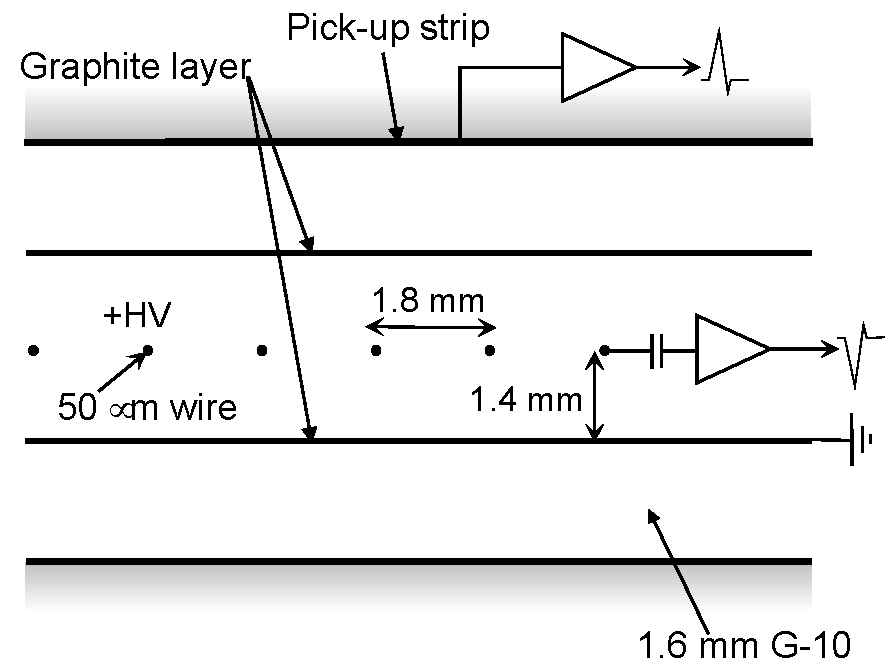
\includegraphics[clip, width=8cm]{fig/2/TGC_anode_wire.pdf}
  \caption{TGC検出器の構造~\cite{Aad:1129811}。}
  \label{fig:2-19}
\end{figure}

\begin{figure}[h]
  \centering
  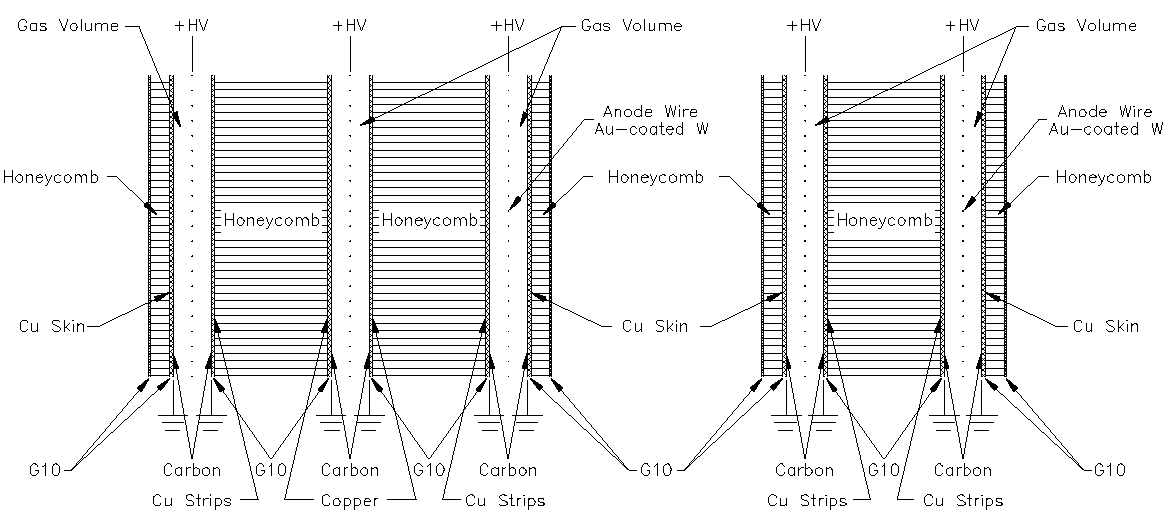
\includegraphics[clip, width=10cm]{fig/2/TGC_construction.pdf}
  \caption{boublet構造(左)とtriplet構造(右)~\cite{Aad:1129811}。}
  \label{fig:2-20}
\end{figure}

\subsubsection{Monitored Drift Tube (MDT)}
MDTはバレル領域、エンドキャップ領域両方に設置されており、35$\mu$mと位置分解能が高いので精密測定に用いられる検出器である。
MDTのドリフトチューブの構造を図~\ref{fig:2-21}に示す。
MDTはArと$CO_{2}$ガスが93 : 7の割合で充填された半径27.979mmのドリフトチューブで構成され、チューブの中心のワイヤーには3080Vの電圧がかけられているので、荷電粒子が通過することによって電離した電子がワイヤーに集められる。
荷電粒子の通過位置は、電子のドリフト距離から求めたドリフトサークルの接線である。
また電子の最大ドリフト時間は約700nsである。

\begin{figure}[h]
  \centering
  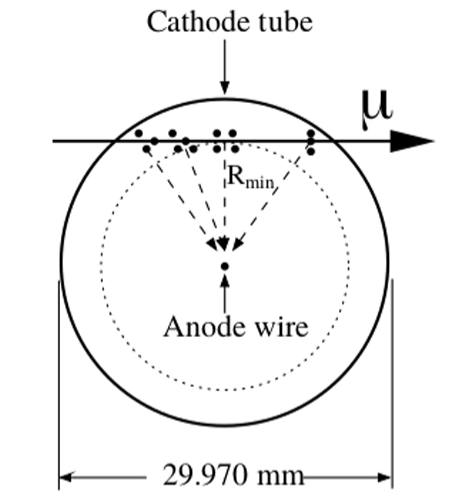
\includegraphics[clip, width=8cm]{fig/2/mdt_driftTube.png}
  \caption{MDTのドリフトチューブの構造~\cite{Aad:1129811}。}
  \label{fig:2-21}
\end{figure}

MDTは図~\ref{fig:2-22}で表されるように、ドリフトチューブ4レイヤーまたは3レイヤーを2層重ねた構造になっている。
MDTはバレル領域では長方形、エンドキャップ領域では台形であり、ドリフトチューブは$\phi$方向に沿って並べられているので、バレル領域で$z$方向、エンドキャップ領域で$R$方向のみ測定可能である。

\begin{figure}[h]
  \centering
  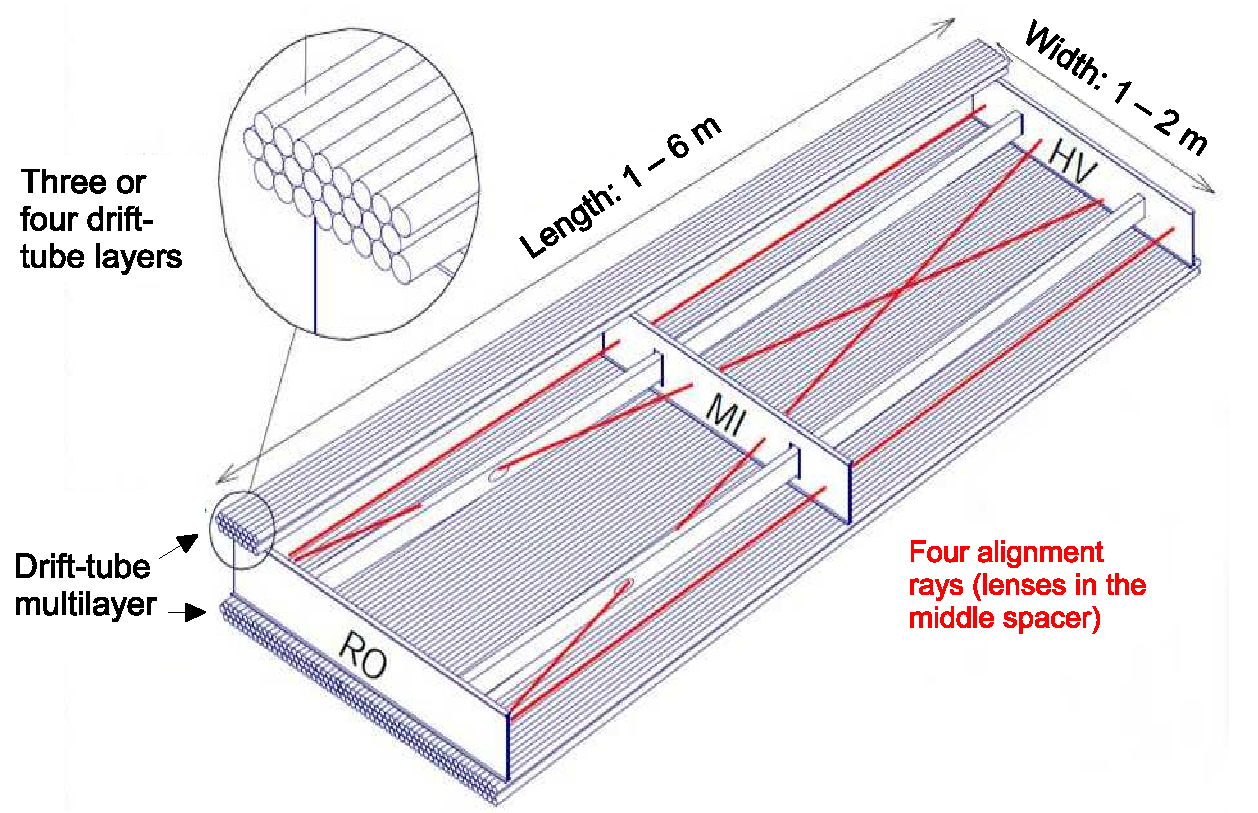
\includegraphics[clip, width=8cm]{fig/2/MDT_chamber_schematics_2.pdf}
  \caption{MDTの構造~\cite{Aad:1129811}。}
  \label{fig:2-22}
\end{figure}

\subsubsection{New Small Wheel (NSW)}
NSWはRun-3よりLHCのルミノシティ増加に伴う高ヒットレート状況下での飛跡測定効率の向上とミューオントリガーの改良を目的として、エンドキャップ領域の磁場領域よりも内側に新たに導入された検出器である。
図~\ref{fig:2-23}にNSWの全体図を示す。
NSWはトリガー用のsmall-strip TGC(sTGC)と精密測定用のMicroMegas(MM)の2種類の検出器をそれぞれ8層ずつ組み合わせた構造をしている。
衝突点側から、sTGC~4層、MM~4層、MM~4層、sTGC~4層の順に16層配置されている。

\begin{figure}[h]
  \centering
  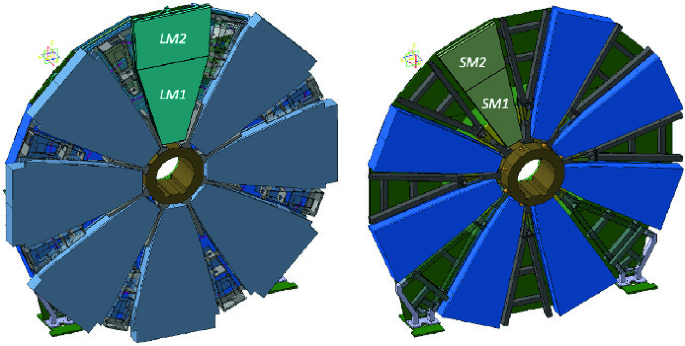
\includegraphics[clip, width=10cm]{fig/2/NSW_structure.png}
  \caption{NSWの全体図\cite{article:ATLASNSWTDR}。左がLarge~Station、右がSmall~Station。}
  \label{fig:2-23}
\end{figure}

sTGCの構造を図~\ref{fig:2-24}に示す。
sTGCでは$\eta$方向と$\phi$方向の測定を、それぞれストリップとワイヤーを用いて行う。
ワイヤーのピッチ幅は1.8mm、ワイヤー平面から1.4mmの距離にある2つのカソード面に挟まれた構造になっている。
カソード面の裏には片側にはパッド、もう一方にワイヤーと垂直にストリップが配置されている。
ストリップのピッチ幅は3.2mmである。ATLASで用いられているTGCと比べてはるかに小さいため、位置分解能が高くsmall-strip~TGCと呼ばれている。

\begin{figure}[h]
  \centering
  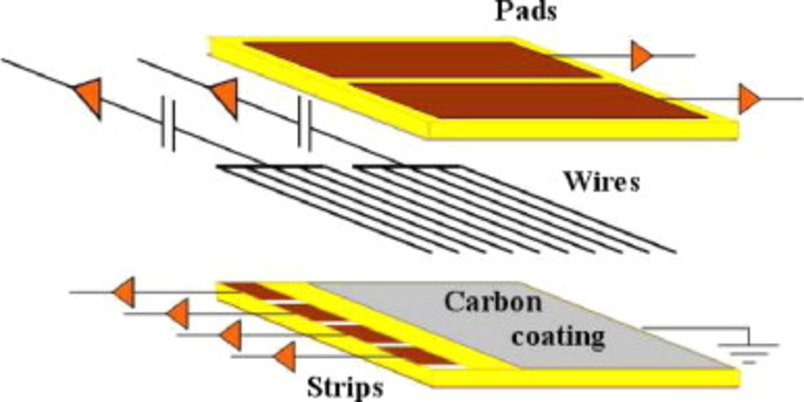
\includegraphics[clip, width=9cm]{fig/2/stgc-structure.pdf}
  \caption{sTGCの構造\cite{article:ATLASNSWTDR}。}
  \label{fig:2-24}
\end{figure}

MMの構造を図~\ref{fig:2-25}に示す。
MMはドリフト電極とガスギャップ、薄い金属メッシュ、増幅領域、読み出し電極で構成されている。ガスギャップは厚さ5mmで、Arと$CO_{2}$が93 : 7で混合されたガスで充填されている。
荷電粒子がMMを通過することで生じた電子がメッシュにドリフトし、メッシュを通過した後で雪崩増幅を起こし、読み出し電極に到達することで入射粒子の位置を特定する。
雪崩増幅で生じたイオンは電子と反対方向に移動し、メッシュに戻る。増幅領域が100$\mu$と他の検出器に比べて狭く、イオンの回収を非常に高速でできるため、高ヒットレート下での読み出しに適した検出器である。
MMは1つの~sectorに8層設置されるが、2次元読み出しを可能にするために4層でストリップを底面に平行に、残りの4層では$\pm15^\circ$ずつ傾けて配置している(図~\ref{fig:2-26})。並行な層をX層、傾けて配置された層をU(V)層と呼ぶ。

\begin{figure}[h]
  \centering
  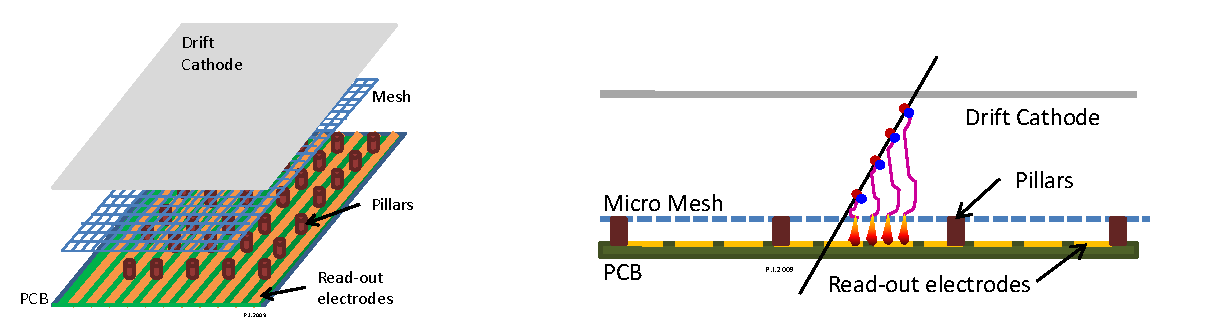
\includegraphics[clip, width=13cm]{fig/2/mm-structure.pdf}
  \caption{MMの構造\cite{article:ATLASNSWTDR}。}
  \label{fig:2-25}
\end{figure}

\begin{figure}[h]
  \centering
  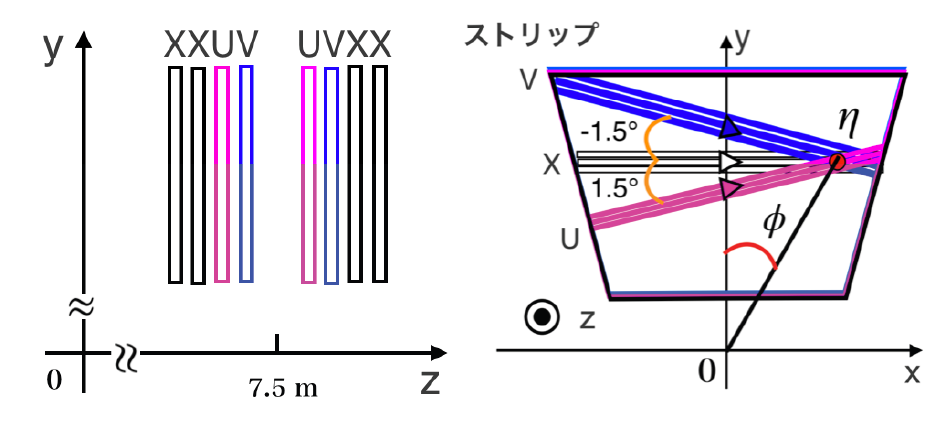
\includegraphics[clip, width=11cm]{fig/2/mm_stereolayer.png}
  \caption{MM$y−z$平面におけるX,U,V 層の並びと$x−y$平面で見た各層のストリップの配置\cite{article:kumaoka}。}
  \label{fig:2-26}
\end{figure}